% -----------------------------------------------
% Template for ISMIR Papers
% 2018 version, based on previous ISMIR templates

% Requirements :
% * 6+n page length maximum
% * 4MB maximum file size
% * Copyright note must appear in the bottom left corner of first page
% * Clearer statement about citing own work in anonymized submission
% (see conference website for additional details)
% -----------------------------------------------

\documentclass{article}
\usepackage{ismir,amsmath,cite,url}
\usepackage{graphicx}
\usepackage{color}
\usepackage{multirow}

% Title.
% ------
\title{From labeled to unlabeled data -- on data challenge in automatic drum transcription}

% Note: Please do NOT use \thanks or a \footnote in any of the author markup

% Single address
% To use with only one author or several with the same address
% ---------------
%\oneauthor
% {Chih-Wei Wu and Alexander Lerch}
% {Center for Music Technology, Georgia Institute of Technology\\ {\tt \{ cwu307, alexander.lerch\}@gatech.edu}}

% Two addresses
% --------------
%\twoauthors
%  {First author} {School \\ Department}
%  {Second author} {Company \\ Address}

%% To make customize author list in Creative Common license, uncomment and customize the next line
%  \def\authorname{First Author, Second Author}


% Three addresses
% --------------
\threeauthors
  {First Author} {Affiliation1 \\ {\tt author1@ismir.edu}}
  {Second Author} {\bf Retain these fake authors in\\\bf submission to preserve the formatting}
  {Third Author} {Affiliation3 \\ {\tt author3@ismir.edu}}

%% To make customize author list in Creative Common license, uncomment and customize the next line
%  \def\authorname{First Author, Second Author, Third Author}

% Four or more addresses
% OR alternative format for large number of co-authors
% ------------
%\multauthor
%{First author$^1$ \hspace{1cm} Second author$^1$ \hspace{1cm} Third author$^2$} { \bfseries{Fourth author$^3$ \hspace{1cm} Fifth author$^2$ \hspace{1cm} Sixth author$^1$}\\
%  $^1$ Department of Computer Science, University , Country\\
%$^2$ International Laboratories, City, Country\\
%$^3$  Company, Address\\
%{\tt\small CorrespondenceAuthor@ismir.edu, PossibleOtherAuthor@ismir.edu}
%}
%\def\authorname{First author, Second author, Third author, Fourth author, Fifth author, Sixth author}


\sloppy % please retain sloppy command for improved formatting

\begin{document}

%
\maketitle
%
\begin{abstract}
Place holder
\end{abstract}
%
\section{Introduction}\label{sec:introduction}

place holder
%
\section{Related Work}
%
place holder
%
\subsection{Automatic Drum Transcription}
% talk about automatic drum transcription
\subsection{Learning from Unlabeled Data}
% talk about learning from unlabeled data
%
\section{Method}
% first, start with an overview figure that shows the main idea of this paper on integrating unlabeled data
\subsection{System Overview}
\begin{figure}
\centering
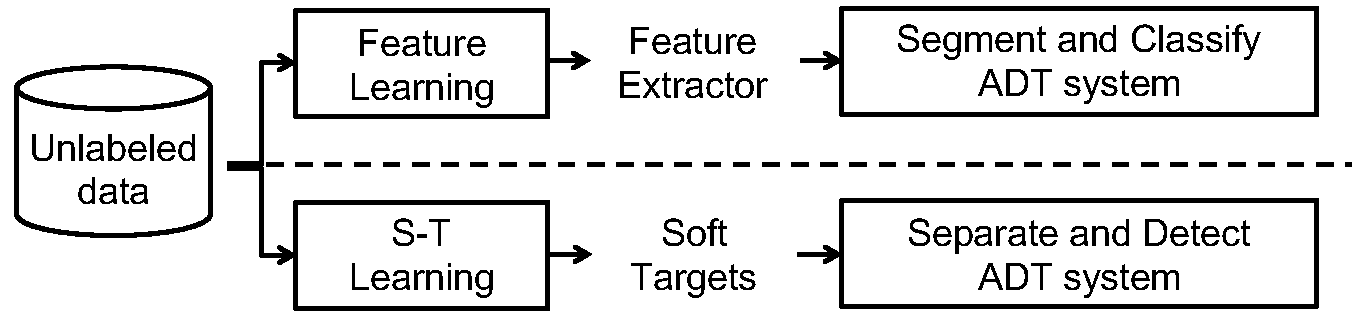
\includegraphics[width = \columnwidth]{./figs/paradigms_overview.pdf}
\caption{The flowchart of the proposed methods for integrating unlabeled data to two major ADT approaches}
\label{fig:flowchart}
\end{figure}


\subsection{Feature Learning}
% zoom in to feature learning based method
\begin{figure}
\centering
\includegraphics[width = \columnwidth]{./figs/featurelearningSys.pdf}
\caption{The flowchart of the feature learning paradigm for ADT}
\label{fig:featureLearningFlow}
\end{figure}



\subsection{Student Teacher Learning}
% zoom in to student teacher learning method
\begin{figure}
\centering
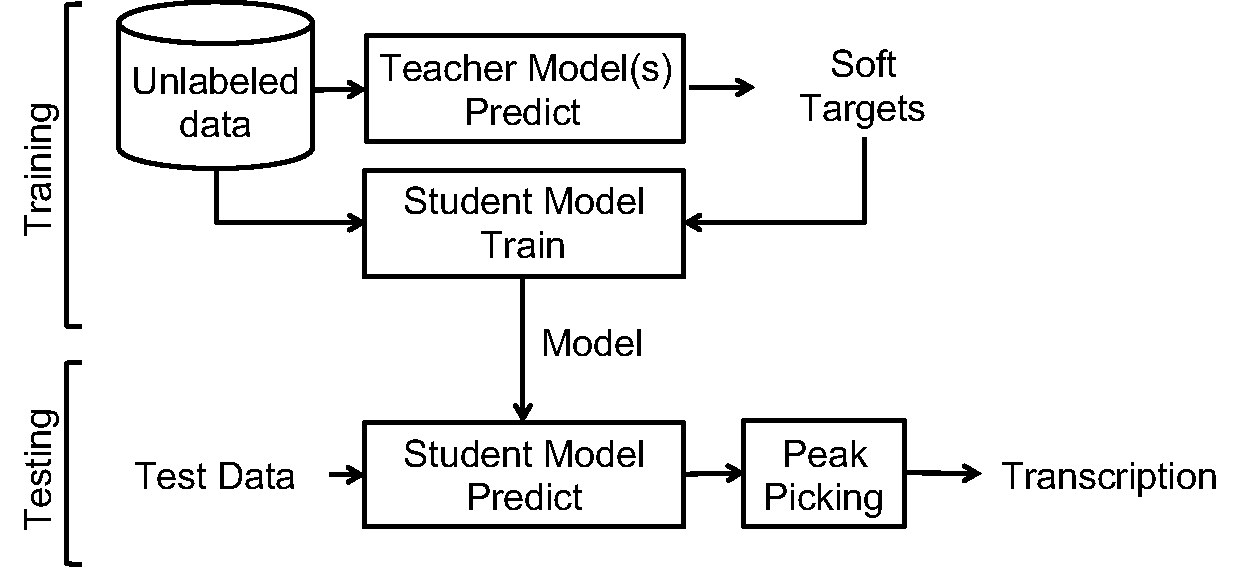
\includegraphics[width = \columnwidth]{./figs/studentTeacherSys.pdf}
\caption{The flowchart of the student-teacher learning paradigm for ADT}
\label{fig:featureLearningFlow}
\end{figure}




\subsection{Implementation}


\section{Experiment}

\subsection{Unlabeled Dataset}

\subsection{Labeled Dataset}

\subsection{Experiment Setup}

\subsection{Metrics}

\textit{mir\_eval}, a python library of commonly used MIR metrics is used for implementing the above mentioned metrics \cite{Raffel2014}. 

\subsection{Results}

% E1: averaged across systems: show the difficulty of the datasets


% E2: results of the feature learning systems
% trained is always better than random except hh
% sd always improved
\begin{table}[]
\centering
\label{my-label}
\begin{tabular}{lllll}
\hline
\multicolumn{2}{l}{\textbf{Experiments}}             & \multicolumn{3}{l}{\textbf{Averaged F-measure}} \\ \hline
\textbf{Role} & \multicolumn{1}{l|}{\textbf{System}} & \textbf{HH}   & \textbf{BD}    & \textbf{SD}    \\ \hline
Baseline      & \multicolumn{1}{l|}{MFCC}            & 0.61          & \textbf{0.62}  & 0.40           \\
Baseline      & \multicolumn{1}{l|}{CONV\_RANDOM}    & 0.61          & 0.54           & 0.39           \\
Proposed      & \multicolumn{1}{l|}{CONV\_AE}        & 0.61          & \textbf{0.62}  & \textbf{0.42}  \\
Proposed      & \multicolumn{1}{l|}{CONV\_DAE}       & 0.61          & 0.61           & \textbf{0.42}  \\ \hline
\end{tabular}
\caption{Evaluation results of the feature-learning-paradigm-based systems. The reported results are the averaged F-measure across four different labeled datasets}
\end{table}
% E3: results of the student-teacher systems
% discuss the varying dataset size vs. results
% criteria for selecting unlabeled data?
\begin{table}[]
\centering
\label{my-label}
\begin{tabular}{lllll}
\hline
\multicolumn{2}{l}{\textbf{Experiments}}                    & \multicolumn{3}{l}{\textbf{Averaged F-measure}} \\ \hline
\textbf{Role} & \multicolumn{1}{l|}{\textbf{System}}        & \textbf{HH}    & \textbf{BD}    & \textbf{SD}   \\ \hline
Teacher       & \multicolumn{1}{l|}{PFNMF (SMT)}            & 0.47           & 0.61           & \textbf{0.45} \\
Teacher       & \multicolumn{1}{l|}{PFNMF (200D)}           & 0.47           & \textbf{0.67}  & 0.40          \\
Student       & \multicolumn{1}{l|}{FC\_200}                & \textbf{0.56}  & 0.57           & 0.44          \\
Student       & \multicolumn{1}{l|}{FC\_1330}               & 0.53           & 0.59           & 0.42          \\
Student       & \multicolumn{1}{l|}{FC\_1330 (ALT)} & 0.55           & 0.58           & 0.44          \\ \hline
\end{tabular}
\caption{Evaluation results of the student-teacher-paradigm-based systems. The reported results are the averaged F-measure across four different labeled datasets}
\end{table}


% additional analysis goes here
\begin{table*}[]
\centering
\begin{tabular}{cccccccc}
\hline
\multicolumn{2}{c}{\textbf{\begin{tabular}[c]{@{}c@{}}Compared \\ Systems\end{tabular}}} & \multirow{2}{*}{\textbf{Instrument}} & \multirow{2}{*}{\textbf{Paradigm}} & \multicolumn{2}{c}{\textbf{\begin{tabular}[c]{@{}c@{}}Improvement\\ Check\end{tabular}}}     & \multicolumn{2}{c}{\textbf{\begin{tabular}[c]{@{}c@{}}Deterioration\\ Check\end{tabular}}}   \\ \cline{1-2} \cline{5-8} 
\textbf{Test}                               & \textbf{Ref}                               &                                      &                                    & \textbf{\# Files} & \textbf{\begin{tabular}[c]{@{}c@{}}Avg. Diff\\ (F-measure)\end{tabular}} & \textbf{\# Files} & \textbf{\begin{tabular}[c]{@{}c@{}}Avg. Diff\\ (F-measure)\end{tabular}} \\ \hline
CONV\_AE                                    & MFCC                                       & SD                                   & Feature Learning                   & 70/137            & 6.5\%                                                                    & 40/137            & -4.6\%                                                                   \\
FC\_200                                     & PFNMF (SMT)                                & HH                                   & S-T Learning                       & 78/137            & 13.8\%                                                                   & 44/137            & -7.6\%                                                                   \\ \hline
\end{tabular}
\caption{Significance check of the most improved pair from each paradigm. Note that the differences between both pairs are statistically significant (p << 0.05)}
\label{my-label}
\end{table*}

% finally, compare two paradigms (pool the best systems from each)
% the differences between two systems are not statistically significant on all instruments
% definitely mention the additional need of labeled data in feature learning 
% so student  teacher is slightly favored for it requires less labeled data

% example from the MIREX 2005 File


\section{Discussion}






\section{Conclusion}


% For bibtex users:
\bibliography{cw_ismir2018_ref.bib}

% For non bibtex users:
%\begin{thebibliography}{citations}
%
%\bibitem {Author:00}
%E. Author.
%``The Title of the Conference Paper,''
%{\it Proceedings of the International Symposium
%on Music Information Retrieval}, pp.~000--111, 2000.
%
%\bibitem{Someone:10}
%A. Someone, B. Someone, and C. Someone.
%``The Title of the Journal Paper,''
%{\it Journal of New Music Research},
%Vol.~A, No.~B, pp.~111--222, 2010.
%
%\bibitem{Someone:04} X. Someone and Y. Someone. {\it Title of the Book},
%    Editorial Acme, Porto, 2012.
%
%\end{thebibliography}

\end{document}
